\chapter{Distributions of Sampling Statistics}


\begin{flushright}
	\textit{``Just find a way to jam it into the Central Limit Theorem"}
\end{flushright}

Most real world populations are intractably large and the statistics of the entire population are impossible to arrive at using brute-force computation. The use of a well-drawn sample to estimate the statistics of the underlying population is the most-used workaround to this problem.

\textbf{Random sample} : A set of random variables which are independent and have a common distribution $ F $. When $ F $ is only specified up to some parameters that are not known, it is possible to estimate these parameters using the statistics of the random sample.

Depending on whether any information about the form of $ F $ is known, this is called either a  \textit{parametric} inference problem, or a \textit{non-parametric} inference problem. An example of the latter is knowing only whether $ F $ is continuous or discrete and nothing further.

\textbf{Statistic} : A RV which is determined by the random sample instead of the underlying population. The two most interesting statistics are the sample mean and the sample variance.

\textbf{Sample mean} : Consider a population with mean $ \mu $ and variance $ \sigma $, without any information about the specific probability distribution. In contrast to the population mean and variance, the \textit{sample mean} of a random sample $ \left\{X_i\right\} $ is defined as

\begin{align}
	\overline{X} &= \frac{X_1 + X_2 + \dots + X_n}{n}
\end{align}

$ \overline{X} $ is also an RV, whose expected value and variance are

\begin{align}
	\mathbb{E}[\overline{X}] &= \frac{1}{n}\ \left(\mathbb{E}[X_1] + \dots + \mathbb{E}[X_n]\right) = \mu \\
	%
	\mathrm{Var}(\overline{X}) &= \frac{1}{n^2}\ \left[\mathrm{Var}(X_1) + \dots + \mathrm{Var}(X_n)\right] = \frac{\sigma^2}{n}
\end{align}

The sample mean from an underlying standard normal population for different values of sample size, is itself a normal RV with spread decreasing as $ n $ increases.

\begin{figure}[H]
	\centering
	\begin{tikzpicture}
		\begin{axis}[width = 0.75\textwidth,xlabel=$\overline{X}$, ylabel=$ f(\overline{X}) $, grid = both, xmin = -4, xmax = 4]
			\addplot[thick, smooth, draw=blue][name path = f2, domain = -5:5]{(1/sqrt(2*pi))*e^(-0.5*x*x)};
			\addplot[thick, smooth, draw=OliveGreen][name path = f3, domain = -5:5]{(1/sqrt(pi))*e^(-0.5*2*x*x)};
			\addplot[thick, smooth, draw=Dandelion][name path = f4, domain = -5:5]{(1/sqrt(0.5*pi))*e^(-0.5*4*x*x)};
			\addplot[thick, smooth, draw=red][name path = f5, domain = -5:5]{(1/sqrt(0.2*pi))*e^(-0.5*10*x*x)};
			\legend{$n=1$,$n=2$,$n=4$, $n=10$}
		\end{axis}
	\end{tikzpicture}
\end{figure}

\textbf{Central Limit Theorem} : Let $ \left\{X_i\right\} $ be independent identically distributed RV having the same mean $ \mu $ and variance $ \sigma^2 $.

In the limit of large $ n $, the distribution of $ \sum X_i $ is approximately normal with mean $ n\mu $ and variance $ n\sigma^2 $, regardless of the probability distribution of the individual $ X_i $ 

\begin{align}
	\frac{X_1 + X_2 + \dots + X_n - n\mu}{\sqrt{n}\ \sigma} &\sim Z
\end{align}

Consider the specific case of a binomial RV with parameters $ (n, p) $. This is decomposed into a set of $ n $ binary indicator RVs. Then for large $ n $,

\begin{align}
	X &= X_1 + X_2 + \dots + X_n \nonumber \\
	%
	\mathbb{E}[X_i] &= p \nonumber \\
	%
	\mathrm{Var}(X_i) &= (1-p) \nonumber \\
	%
	\frac{X - np}{\sqrt{np(1-p)}} & \sim Z 
\end{align}

\begin{figure}[!h]
	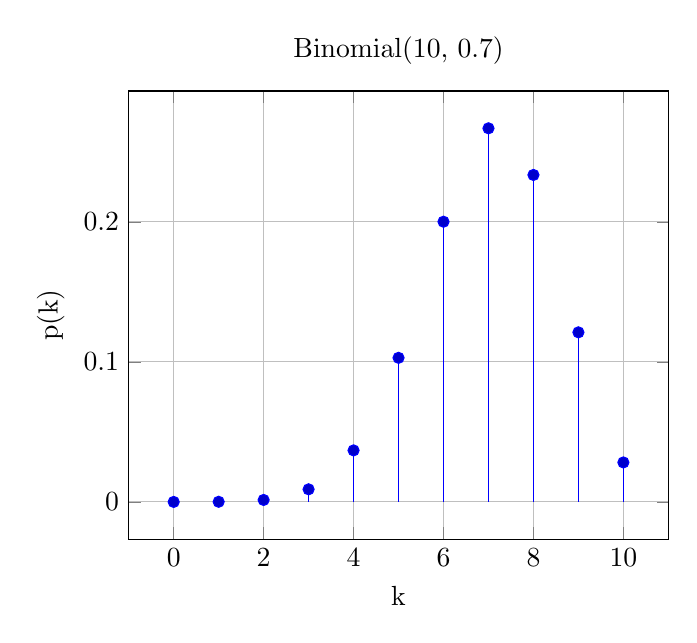
\begin{tikzpicture}
		\begin{axis}[grid = both,
			xlabel = k, ylabel = p(k), title = {Binomial(10, 0.7)}]
			\addplot+[ycomb] plot coordinates {( 0 , 0.0 ) ( 1 , 0.0001 ) ( 2 , 0.0014 ) ( 3 , 0.009 ) ( 4 , 0.0368 ) ( 5 , 0.1029 ) ( 6 , 0.2001 ) ( 7 , 0.2668 ) ( 8 , 0.2335 ) ( 9 , 0.1211 ) ( 10 , 0.0282 ) 
			 };  
		\end{axis} 
	\end{tikzpicture}
	%
	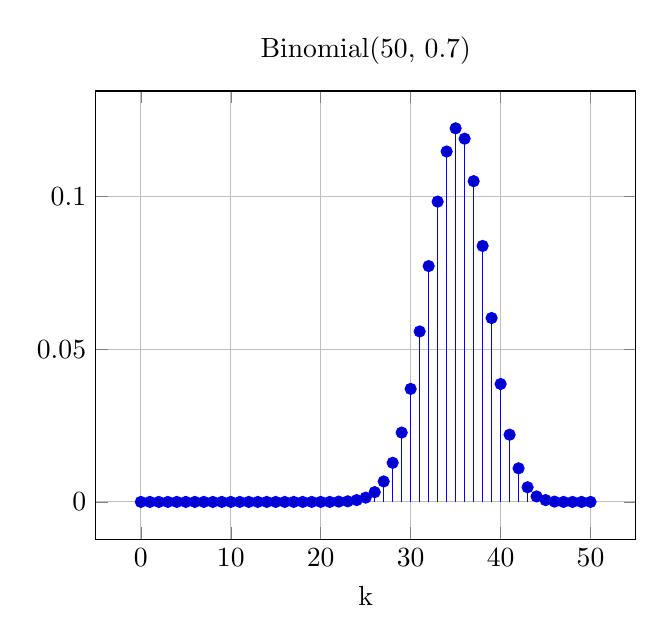
\begin{tikzpicture}
		\begin{axis}[grid = both, yticklabel style={
				/pgf/number format/fixed,
				/pgf/number format/precision=2
			},
			xlabel = k, title = {Binomial(50, 0.7)}]
			\addplot+[ycomb] plot coordinates {( 0 , 0.0 ) ( 1 , 0.0 ) ( 2 , 0.0 ) ( 3 , 0.0 ) ( 4 , 0.0 ) ( 5 , 0.0 ) ( 6 , 0.0 ) ( 7 , 0.0 ) ( 8 , 0.0 ) ( 9 , 0.0 ) ( 10 , 0.0 ) ( 11 , 0.0 ) ( 12 , 0.0 ) ( 13 , 0.0 ) ( 14 , 0.0 ) ( 15 , 0.0 ) ( 16 , 0.0 ) ( 17 , 0.0 ) ( 18 , 0.0 ) ( 19 , 0.0 ) ( 20 , 0.0 ) ( 21 , 0.0 ) ( 22 , 0.0001 ) ( 23 , 0.0002 ) ( 24 , 0.0006 ) ( 25 , 0.0014 ) ( 26 , 0.0032 ) ( 27 , 0.0067 ) ( 28 , 0.0128 ) ( 29 , 0.0227 ) ( 30 , 0.037 ) ( 31 , 0.0558 ) ( 32 , 0.0772 ) ( 33 , 0.0983 ) ( 34 , 0.1147 ) ( 35 , 0.1223 ) ( 36 , 0.1189 ) ( 37 , 0.105 ) ( 38 , 0.0838 ) ( 39 , 0.0602 ) ( 40 , 0.0386 ) ( 41 , 0.022 ) ( 42 , 0.011 ) ( 43 , 0.0048 ) ( 44 , 0.0018 ) ( 45 , 0.0006 ) ( 46 , 0.0001 ) ( 47 , 0.0 ) ( 48 , 0.0 ) ( 49 , 0.0 ) ( 50 , 0.0 ) 
			};  
		\end{axis} 
	\end{tikzpicture}
\end{figure} 

While the Poisson approximation to a Binomial RV is good for large $ n $ and small $ p $, this normal approximation is only good for large values of $ \sqrt{np(1-p)} $, with this value by convention being $ \geq 10 $.

The sample mean also obeys the central limit theorem for large values of sample size $ n $ to give,

\begin{align}
	\frac{\overline{X} - \mu}{\sigma / \sqrt{n}} &\sim Z
\end{align}

By convention, a sample size of at least $ 30 $ is needed to ensure that the sample mean will be approximately normal regardless of the underlying probability distribution. This minimum sample size is much smaller for specific distributions such as a normal RV ($ n \geq 1 $) and an exponential RV ($ n \geq 5 $)


\begin{figure}[H]
	\centering
	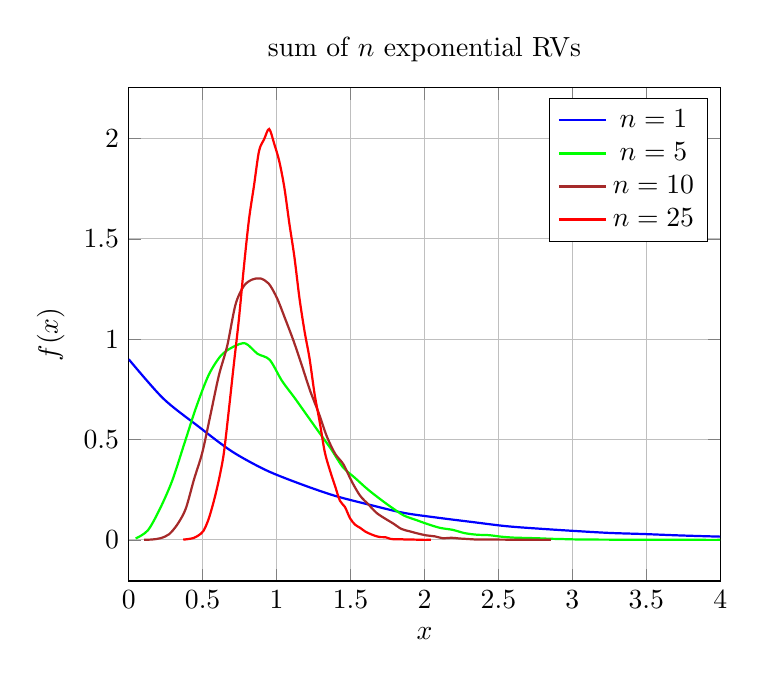
\begin{tikzpicture}
	\begin{axis}[width = 0.75\textwidth,grid = both, xmax = 4.0, xmin = 0,
		xlabel = $ x $, ylabel=$ f(x) $, title = sum of $ n $ exponential RVs]

		\addplot[smooth, thick, color = blue] plot coordinates {
			(0.0, 0.9003) (0.2322, 0.7054) (0.4643, 0.5692) (0.6965, 0.4414) (0.9286, 0.3473) (1.1607, 0.2788) (1.3929, 0.2199) (1.625, 0.1757) (1.8572, 0.1349) (2.0893, 0.1105) (2.3215, 0.0891) (2.5536, 0.0682) (2.7858, 0.0553) (3.0179, 0.0443) (3.2501, 0.0346) (3.4822, 0.0291) (3.7144, 0.0224) (3.9465, 0.0172) (4.1787, 0.013) (4.4108, 0.0109) (4.643, 0.0083) (4.8751, 0.0069) (5.1073, 0.0053) (5.3394, 0.0037) (5.5716, 0.0036) (5.8037, 0.0027) (6.0359, 0.0019) (6.268, 0.0015) (6.5002, 0.0012) (6.7323, 0.0009) (6.9645, 0.0009) (7.1966, 0.0006) (7.4288, 0.0006) (7.6609, 0.0002) (7.8931, 0.0002) (8.1252, 0.0002) (8.3574, 0.0002) (8.5895, 0.0003) (8.8217, 0.0001) (9.0538, 0.0002) (9.286, 0.0001) (9.5181, 0.0002) (9.7502, 0.0) (9.9824, 0.0) (10.2145, 0.0001) (10.4467, 0.0) (10.6788, 0.0) (10.911, 0.0) (11.1431, 0.0) (11.3753, 0.0001)
			
		}; 
		\addplot[smooth, thick, color = green] plot coordinates {
			(0.0473, 0.007) (0.1297, 0.0475) (0.2121, 0.1563) (0.2945, 0.2957) (0.3769, 0.4815) (0.4593, 0.6674) (0.5417, 0.823) (0.6241, 0.9185) (0.7064, 0.9618) (0.7888, 0.9792) (0.8712, 0.9273) (0.9536, 0.897) (1.036, 0.7929) (1.1184, 0.7112) (1.2008, 0.6257) (1.2832, 0.5401) (1.3656, 0.4557) (1.448, 0.3626) (1.5304, 0.3085) (1.6128, 0.254) (1.6952, 0.206) (1.7776, 0.1617) (1.86, 0.1217) (1.9424, 0.0994) (2.0248, 0.0776) (2.1071, 0.0595) (2.1895, 0.0501) (2.2719, 0.0336) (2.3543, 0.0257) (2.4367, 0.0234) (2.5191, 0.0159) (2.6015, 0.0113) (2.6839, 0.0096) (2.7663, 0.008) (2.8487, 0.0055) (2.9311, 0.004) (3.0135, 0.0024) (3.0959, 0.0022) (3.1783, 0.0013) (3.2607, 0.0011) (3.3431, 0.0007) (3.4255, 0.0007) (3.5078, 0.0006) (3.5902, 0.0001) (3.6726, 0.0006) (3.755, 0.0004) (3.8374, 0.0004) (3.9198, 0.0) (4.0022, 0.0001) (4.0846, 0.0002)
		}; 
		\addplot[smooth, thick, color = Brown] plot coordinates {
			(0.1048, 0.0005) (0.1609, 0.002) (0.2171, 0.0087) (0.2732, 0.0282) (0.3293, 0.0773) (0.3854, 0.1545) (0.4416, 0.3015) (0.4977, 0.4353) (0.5538, 0.6265) (0.6099, 0.82) (0.666, 0.9665) (0.7222, 1.1726) (0.7783, 1.2649) (0.8344, 1.2972) (0.8905, 1.3027) (0.9467, 1.2772) (1.0028, 1.2049) (1.0589, 1.1001) (1.115, 0.991) (1.1711, 0.8686) (1.2273, 0.742) (1.2834, 0.635) (1.3395, 0.516) (1.3956, 0.4294) (1.4518, 0.3765) (1.5079, 0.2915) (1.564, 0.2209) (1.6201, 0.1771) (1.6763, 0.1342) (1.7324, 0.1066) (1.7885, 0.0816) (1.8446, 0.0542) (1.9007, 0.0424) (1.9569, 0.0314) (2.013, 0.0223) (2.0691, 0.0176) (2.1252, 0.008) (2.1814, 0.0105) (2.2375, 0.0068) (2.2936, 0.0043) (2.3497, 0.0018) (2.4058, 0.0023) (2.462, 0.0018) (2.5181, 0.0012) (2.5742, 0.0011) (2.6303, 0.0009) (2.6865, 0.0002) (2.7426, 0.0002) (2.7987, 0.0) (2.8548, 0.0004)
		};
		\addplot[smooth, thick, color = red] plot coordinates {
			(0.3687, 0.0012) (0.4029, 0.0041) (0.4371, 0.0091) (0.4712, 0.0219) (0.5054, 0.0448) (0.5396, 0.1021) (0.5738, 0.1884) (0.6079, 0.2929) (0.6421, 0.4258) (0.6763, 0.6417) (0.7105, 0.8726) (0.7446, 1.0961) (0.7788, 1.3592) (0.813, 1.595) (0.8472, 1.7651) (0.8813, 1.938) (0.9155, 1.9959) (0.9497, 2.0477) (0.9839, 1.9737) (1.018, 1.8871) (1.0522, 1.7569) (1.0864, 1.5763) (1.1206, 1.4089) (1.1547, 1.2044) (1.1889, 1.04) (1.2231, 0.903) (1.2573, 0.7251) (1.2914, 0.5879) (1.3256, 0.4386) (1.3598, 0.3485) (1.394, 0.2718) (1.4281, 0.1955) (1.4623, 0.1639) (1.4965, 0.108) (1.5307, 0.0758) (1.5648, 0.06) (1.599, 0.0418) (1.6332, 0.0296) (1.6674, 0.0199) (1.7015, 0.0138) (1.7357, 0.0132) (1.7699, 0.005) (1.804, 0.0029) (1.8382, 0.0035) (1.8724, 0.0015) (1.9066, 0.0015) (1.9407, 0.0012) (1.9749, 0.0003) (2.0091, 0.0) (2.0433, 0.0006)
			
		};
	\legend{$n=1$,$n=5$,$n=10$, $n=25$}		
	\end{axis} 
	\end{tikzpicture}
\end{figure} 

\textbf{Sample variance} : Using the prior definition of the variance $ S^2 $, a sample drawn from an underlying distribution with parameters $ \mu, \sigma $ and sample mean $ \overline{X} $ has the sample variance $ S^2 $ defined as,

\begin{align}
	S^2 &= \ddfrac{\sum\limits_{i=1}^{n}(X_i - \overline{X})^2}{n-1}
\end{align}

The expected value of the sample variance is found using,

\begin{align}
	\sum\limits_{i=1}^{n}(x_i - \overline{x})^2 &= \sum\limits_{i=1}^{n}(x_i^2) - n\overline{x}^2 \nonumber \\
	%
	\mathbb{E}[X^2] &= \mathrm{Var}(X) + (\mathbb{E}[X])^2 \nonumber 
\end{align}

The derivation of $ \mathbb{E}[S^2] $, using the above relations is as follows,

\begin{align}
	(n-1)\mathbb{E}[S^2] &= \mathbb{E}\left[\sum\limits_{i=1}^{n}X_i^2\right] - n\mathbb{E}[\overline{X}^2] \nonumber \\
	%
	&= n\left[\mathrm{Var}(X_1) + (\mathbb{E}[X_1])^2 - \mathrm{Var}(\overline{X}) - (\mathbb{E}[\overline{X}])^2\right] \nonumber \\
	%
	&= n\sigma^2 + n\mu^2 - n(\sigma^2/n) - n\mu^2 \nonumber \\
	%
	\mathbb{E}[S^2] &= \sigma^2
\end{align}

\textbf{Sampling from a normal population} : For the specific case of samples drawn from an underlying population which is normally distributed $ X_i \sim \mathcal{N}(\mu, \sigma^2) $, the distribution of the sample mean and sample variance is of particular interest for real-world applications.

The sample mean $ \overline{X} $ is itself a normal RV, with mean $ \mu $ and variance $ \sigma^2 / n $ 

The sample variance is independent from the sample mean exclusively when the underlying population is a normal RV, with

\begin{align}
	\frac{(n-1)}{\sigma^2}\ S^2 &\sim \chi^2_{n-1}
\end{align}

As a corollary to the above, a t-distribution with $ (n-1) $ DOF, can be observed from the following combination of the sample mean and sample variance,

\begin{align}
	\frac{\overline{X}- \mu}{\sigma / \sqrt{n}}\ \sqrt{\frac{\sigma^2}{S^2}} &\sim \frac{Z}{\sqrt{\chi^2_{n-1} / (n-1)}} \nonumber \\
	%
	\frac{\sqrt{n}\ (\overline{X}- \mu)}{S} &\sim t_{n-1}
\end{align}

\textbf{Sampling from finite population} : Consider a population of size $ N $, which has a proportion $ p $ of its elements possessing a certain property of interest. A random sample of size $ n $ picked from this population would be equally likely to be any of the possible binomial combinations.

The most common method of successively generating a random sample is to simply select one of the remaining members of the population at random at each step until the desired sample size is reached.

A set of binary indicator RVs $ \left\{X_i\right\} $ which indicate whether the $ i^{th} $ member of the sample possesses the property of interest would then sum up to $ X = \sum X_i $. Note that these $ X_i $ are not independent. Independence of the $ X_i $ is a valid assumption only for $ N \ggg n $

\begin{align}
	P\left\{X_i = 1\right\} &= p \qquad \text{and} \qquad P\left\{X_i = 0\right\} = (1-p)
\end{align}

The sample mean $ \overline{X} $ is the proportion of the sample that has the property of interest. In the limit of large $ N $, $ X $ becomes a binomial RV with parameters $ (n, p) $.

When the sample is not a very small fraction of the population, $ X $ is a hyper-geometric random variable with parameters $ (Np, N(1-p), n) $

Proceeding with the $ N \ggg n $ approximation, $ X $ reduces to a binomial RV.

\begin{align}
	\mathbb{E}[\overline{X}] &= p \\
	%
	\mathrm{Var}(\overline{X}) &= \frac{p(1-p)}{n}
\end{align}

